\section{Appendix and Notes}\label{sec:appendix}
Material referred to in the report but not essential to its argument.

\subsection{Demonstration screenshot}
% Required by the brief: a screenshot of the controller tracking the setpoint, taken during the
% demo with Mr De Maar.

\subsection{Analysis code}
The parameter extraction, gain window, resistor selection and closed-loop simulation were run
with the scripts in \texttt{analysis/}: \texttt{stepfit.py} for the step test fit,
\texttt{design.py} for the gain window, \texttt{bom.py} for the resistor pairs and
\texttt{simloop.py} for the simulated loop including input saturation.

\subsection{Additional figures}
% Raw traces, discarded runs and bench photographs that support the text.

\subsection{Decay test, in full}
In a step test the gain and the time constant come from the same curve, so
an error in one can be absorbed by the other. Returning the input to hover breaks that coupling:
the velocity decays with no final value for the gain to influence. Both logs taken for this purpose
turned out to contain the whole bench session rather than a single event, with $14$ and $28$
separate input changes, so neither is a clean decay and a $36.8$ percent reading taken across them
would be meaningless. One usable segment survives, in \texttt{decay\_3p5\_a}: a hand sweep back to
hover followed by $164\ \mathrm{s}$ undisturbed. Because the input does not land exactly on hover,
the decay is to a non-zero velocity and the final value must be fitted rather than assumed,
\begin{equation}
    v(t) = v_\infty + \left(v_0 - v_\infty\right)e^{-t/T} .
\end{equation}
Fitting all three parameters over $1640$ samples gives $T = 9.163\ \mathrm{s}$ with an rms residual
of $0.113\ \mathrm{m\,s^{-1}}$. That is $3.9$ percent below the $9.537\ \mathrm{s}$ of the step
test, which is the honest size of the disagreement between the two methods and is carried into the
uncertainty below.

The same fit returns a residual velocity of $0.157\ \mathrm{m\,s^{-1}}$. The input over that
segment averaged $2.5080\ \mathrm{V}$, and the identified gain and hover voltage predict
$23.196 \times (2.5080 - 2.5016) = 0.149\ \mathrm{m\,s^{-1}}$. The two agree to
$0.008\ \mathrm{m\,s^{-1}}$. This is the strongest single check in the identification, because it
predicts a small number from two constants measured elsewhere, in a part of the data that played no
part in measuring them.

The second log, \texttt{decay\_3p9\_a}, is discarded rather than averaged in. Its longest
undisturbed stretch shows the velocity rising, not decaying, so it does not describe the experiment
it was recorded for.

\subsection{Error and disturbance transfer functions}
Tracking accuracy and disturbance rejection are separate questions with separate answers, so
each needs its own transfer function.

The error between the setpoint and the position is
\begin{equation}\label{eqn:error_tf}
    \frac{E(s)}{X(s)} = \frac{1}{1 + L(s)} = \frac{s(Ts + 1)}{Ts^2 + s + K_p k A} ,
\end{equation}
and because gravity enters at the plant input, its effect on the output is the plant path over
the same return difference,
\begin{equation}\label{eqn:dist_tf}
    \frac{Y(s)}{D(s)} = \frac{G(s)}{1 + L(s)} = \frac{A}{Ts^2 + s + K_p k A} .
\end{equation}

The loop gain of Equation~\eqref{eqn:loopgain} has exactly one pole at the origin, so the system
is \textbf{type 1}. Applying the final value theorem to Equation~\eqref{eqn:error_tf} for a step
setpoint of size $X_0$,
\begin{equation}\label{eqn:fvt_error}
    e_\infty = \lim_{s \to 0} s \cdot \frac{s(Ts+1)}{Ts^2 + s + K_p k A} \cdot \frac{X_0}{s} = 0 ,
\end{equation}
so the steady-state position error to a step setpoint is zero and proportional control alone is
enough to track it. Applying the same theorem to Equation~\eqref{eqn:dist_tf} for a constant
disturbance of equivalent input magnitude $d$,
\begin{equation}\label{eqn:fvt_dist}
    y_\infty\big|_{\text{grav}}
    = \lim_{s \to 0} s \cdot \frac{A}{Ts^2 + s + K_p k A} \cdot \frac{d}{s}
    = \frac{d}{K_p k} ,
\end{equation}
which is finite but not zero, and shrinks as $K_p$ grows.

The asymmetry between Equations~\eqref{eqn:fvt_error} and~\eqref{eqn:fvt_dist} decides where
the tracking budget goes. Type 1 says one integrator sits in the loop, but what it rejects
depends on where. Here it belongs to the plant, at the same node the disturbance enters, not to
the controller. A setpoint error must pass through the integrator to reach the output, so a
constant error would integrate into an unbounded position and the only consistent steady state
is zero. A constant input disturbance arrives at that node instead, so the proportional gain
fights it directly and finite gain leaves the finite offset of
Equation~\eqref{eqn:fvt_dist}. An integral term would remove it, but that is PI control and
outside this lab. The consequence for Section~\ref{sec:design} is that the whole tracking budget
belongs to the disturbance. In practice the level shift cancels the nominal gravity term, so
what reaches the output is the residual after trimming rather than the full $d$.

\subsection{Circuit simulation, LTspice}
The netlist of \texttt{analysis/spice/controller\_ltspice.cir} was also run in \textsc{LTspice},
independently of the \textsc{ngspice} run reported in Section~\ref{sec:design}, as a check that
the result does not depend on the simulator. Figure~\ref{fig:ltspice} is the DC sweep of the
feedback voltage through the operating point.

\begin{figure}[htbp]
    \centering
    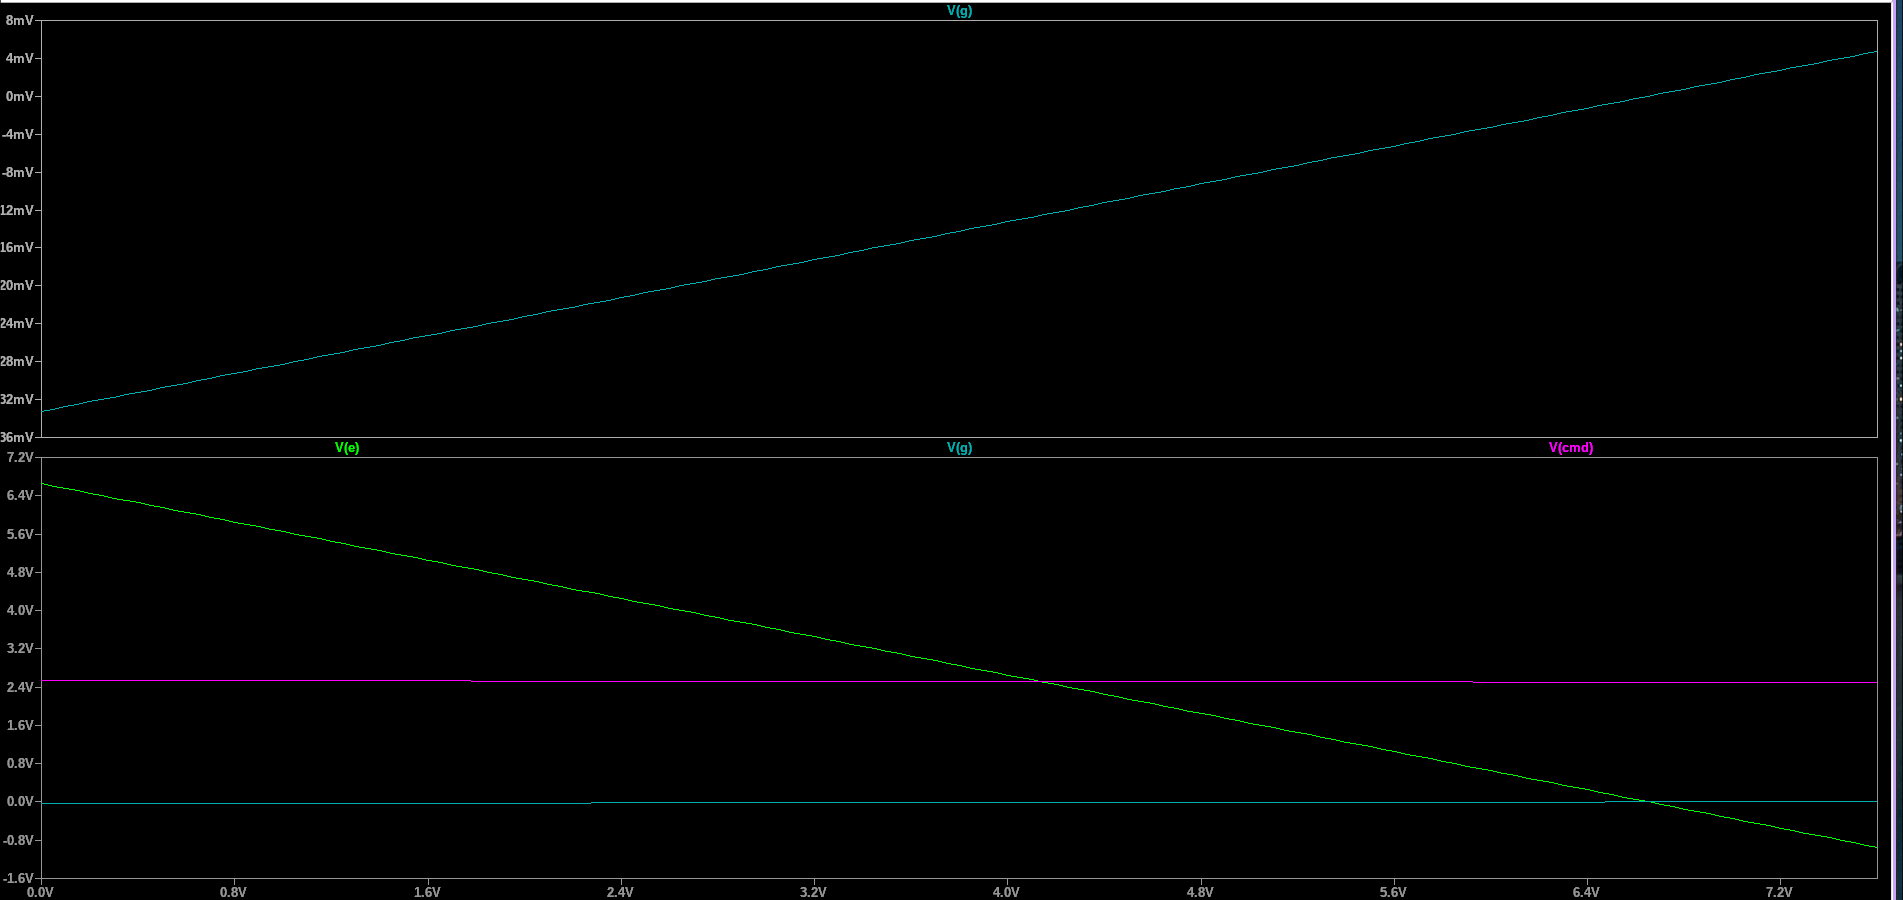
\includegraphics[width=0.92\textwidth]{figures/ltspice_sweep.png}
    \caption{LTspice DC sweep of the built controller. Upper pane: the gain stage output
    $V_g$ rising linearly from $-33\ \mathrm{mV}$ and crossing zero where the feedback equals the
    $6.65\ \mathrm{V}$ setpoint, which is $K_p = 0.005$ with the inversion intact. Lower pane: the
    error $V_e$ falling with unit slope, confirming the difference amplifier subtracts exactly,
    and the command $V_{cmd}$ holding at the hover bias. The command moves only
    $37\ \mathrm{mV}$ across the whole sweep, which is why the $0$ to $5\ \mathrm{V}$ limit never
    binds.}
    \label{fig:ltspice}
\end{figure}

Three stages are verified at once by this one sweep: the subtraction from the slope of $V_e$, the
gain and its sign from the slope of $V_g$, and the level shift from the value of $V_{cmd}$ at zero
error. All three agree with the hand calculations and with \textsc{ngspice}.

\subsection{Bias divider under load, and the circuit simulation}
\paragraph{Loading of the bias divider.} The divider cannot be designed on its own, because the
$10\ \mathrm{k\Omega}$ input resistor of stage 3 loads it. Writing the divider as a Th\'evenin
source $V_{th}$ behind $R_{th} = R_7 \parallel R_8$, the voltage reaching the non-inverting input
is divided again by the stage's own pair, so
\begin{equation}\label{eqn:bias_loaded}
    V_{cmd}\big|_{V_e = 0} = 2 V_{th}\frac{10\ \mathrm{k}}{R_{th} + 20\ \mathrm{k}} .
\end{equation}
An unloaded design giving exactly $2.50\ \mathrm{V}$ would deliver only $2.35\ \mathrm{V}$ once
connected, a $0.15\ \mathrm{V}$ error, which Figure~\ref{fig:robustness_bias} shows would be a
$450$ percent steady-state offset. Solving Equation~\eqref{eqn:bias_loaded} for
$V_{cmd} = 2.500\ \mathrm{V}$ with $R_8 = 1\mathrm{k}2$ gives $R_7 = 5.65\ \mathrm{k\Omega}$,
which is why the upper leg is a $4\mathrm{k}7$ in series with a $2\ \mathrm{k\Omega}$ trimmer
rather than a single fixed part. Keeping the divider impedance near $1\ \mathrm{k\Omega}$ rather
than the $10\ \mathrm{k\Omega}$ used elsewhere also keeps $R_{th}$ small against the
$20\ \mathrm{k\Omega}$ in the denominator, so the trimmer setting moves the level without greatly
changing the loading.

\paragraph{Simulation of the circuit itself.} The three stages were simulated in \textsc{ngspice}
with a behavioural UA741 model (open-loop gain $2\times 10^5$, dominant pole at $5\ \mathrm{Hz}$
for a $1\ \mathrm{MHz}$ gain-bandwidth product, $75\ \Omega$ output). Sweeping the feedback
voltage through the operating point gives an output slope of $+0.005\ \mathrm{V/V}$, confirming
both the magnitude of $K_p$ and that the two inversions cancel, and an output of
$2.504\ \mathrm{V}$ at zero error against the $2.5038\ \mathrm{V}$ predicted by
Equation~\eqref{eqn:bias_loaded}. The netlist is \texttt{analysis/spice/controller.cir}.

\subsection{Sensitivity of the steady-state offset to the bias trim}
\begin{figure}[htbp]
    \centering
    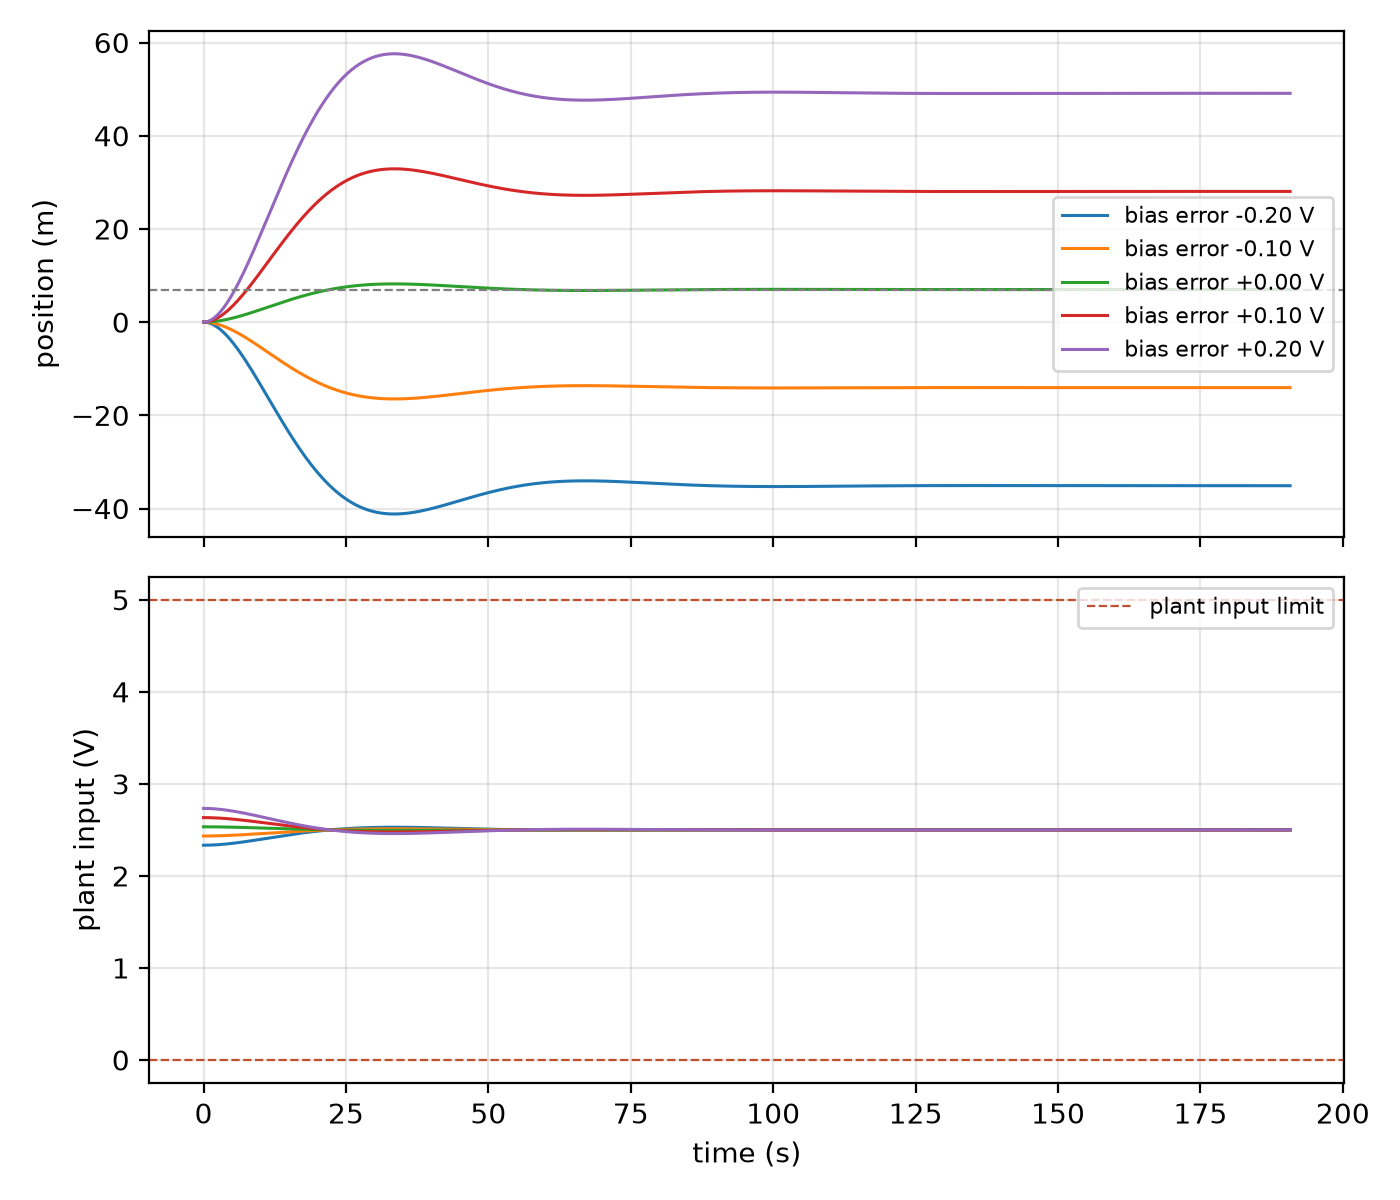
\includegraphics[width=0.55\textwidth]{figures/robustness_bias.png}
    \caption{Bias trim error swept from $0$ to $0.2\ \mathrm{V}$. The offset is proportional to it
    and nothing else: a perfectly trimmed bias leaves $0.01$ percent error, while a
    $0.1\ \mathrm{V}$ error leaves $300$ percent. Overshoot is untouched throughout, since the
    bias enters as a disturbance and not as a change of loop gain.}
    \label{fig:robustness_bias}
\end{figure}

\subsection{Controller gain window at every tolerance corner}
% generated by analysis/design.py, do not edit by hand
\begin{table}[htbp]
  \centering
  \caption{Controller performance at every corner of the tolerance budget, $K_p = 0.005$ nominal. Window 0.005 to 0.006.}
  \label{tab:corners}
  \begin{tabular}{rrrrrrr}
    \toprule
    $T$ (s) & gain factor & $K_{p,\text{eff}}$ & $\zeta$ & Overshoot (\%) & Offset (m) & Kick (V) \\
    \midrule
    8.583 & 0.82 & 0.004 & 0.577 & 10.84 & 0.4780 & 0.03 \\
    8.583 & 1.00 & 0.005 & 0.523 & 14.56 & 0.3920 & 0.04 \\
    8.583 & 1.22 & 0.007 & 0.473 & 18.48 & 0.3213 & 0.04 \\
    9.537 & 0.82 & 0.004 & 0.520 & 14.79 & 0.4780 & 0.03 \\
    9.537 & 1.00 & 0.005 & 0.471 & 18.72 & 0.3920 & 0.04 \\
    9.537 & 1.22 & 0.007 & 0.426 & 22.77 & 0.3213 & 0.04 \\
    10.491 & 0.82 & 0.004 & 0.472 & 18.56 & 0.4780 & 0.03 \\
    10.491 & 1.00 & 0.005 & 0.428 & 22.60 & 0.3920 & 0.04 \\
    10.491 & 1.22 & 0.007 & 0.387 & 26.72 & 0.3213 & 0.04 \\
    \bottomrule
  \end{tabular}
\end{table}


\subsection{Step test runs}
\begin{table}[htbp]
\centering
\begin{tabular}{lrrrr}
\toprule
Run & $V_{in}$ (V) & $V_{in}-V_h$ (V) & $v_\infty$ (m/s) & $A$ \\
\midrule
\texttt{step\_2p9\_a}    & 2.911 & 0.409 & \phantom{0}9.513 & 23.24 \\
\texttt{step\_2p9\_a\_v2} & 2.917 & 0.415 & \phantom{0}9.606 & 23.14 \\
\texttt{step\_3p2\_a}    & 3.212 & 0.711 & 16.460 & 23.15 \\
\texttt{step\_3p2\_a\_v2} & 3.209 & 0.707 & 16.414 & 23.22 \\
\texttt{step\_3p5\_a}    & 3.503 & 1.001 & 23.214 & 23.19 \\
\texttt{step\_3p9\_a}    & 4.004 & 1.502 & 34.887 & 23.22 \\
\texttt{step\_3p9\_a\_v2} & 3.896 & 1.394 & 32.351 & 23.20 \\
\texttt{demaar\_run}     & 5.000 & 2.498 & 57.935 & 23.19 \\
\bottomrule
\end{tabular}
\caption{The eight runs, with $v_\infty$ taken as the slope of a straight line through the last
$20$ percent of each height record rather than from a two-point difference, and $V_{in}$ as the
mean of the input column over the same window. Individual gains span $23.14$ to $23.24$, a spread
of $0.4$ percent across a sixfold range of step size.}
\label{tab:stepruns}
\end{table}

\subsection{Parameter check}
The simulator ships a separate checking tool that scores a submitted $A$, $T$ and sensor constant
against the values the rig was generated from. Three submissions were allowed. They were used as a
sensitivity probe rather than as three guesses, by entering the measured values and then entering
values deliberately displaced from them to see how fast the score falls.

\begin{table}[htbp]
\centering
\caption{Parameter check submissions and returned scores.}
\label{tab:paramcheck}
\begin{tabular}{cccccc}
\hline
Attempt & $A$ & score & $T$ & score & sensor score \\
\hline
1 & 23.300 & 44\% & 10.210 & 22\% & 100\% \\
2 & 23.128 & 54\% & \phantom{0}9.535 & 46\% & 100\% \\
3 & 22.500 & 18\% & \phantom{0}8.600 & \phantom{0}2\% & 100\% \\
\hline
\end{tabular}
\end{table}

Table~\ref{tab:paramcheck} lists the three submissions. The sensor constant was returned exact on every attempt, which is expected: it is read directly
from the ratio of the two logged output columns and involves no fitting.

For $A$ and $T$ the scores are not monotonic in the entered value. Attempt~2 scores higher than
attempt~1, which lies above it, and far higher than attempt~3, which lies below it, so the
checker's values are bracketed by attempts~1 and~3 and sit close to the measured ones. The drop
from attempt~2 to attempt~3 is steep: a $2.7$ percent change in $A$ costs $36$ marks and a $9.8$
percent change in $T$ costs $44$, so the scoring function penalises error far more sharply than a
linear or exponential law fitted to the first two attempts would predict. Attempts~1 and~2 alone
were consistent with a shallow penalty and a target below the measurements; attempt~3 rules that
out. Two points were not enough to identify the scoring function, and the shape assumed from them
was wrong.

The measured values are kept as the identified model. They scored best of the three submissions,
they are bracketed by the attempts either side, and unlike the checker's hidden figures they are
traceable to the logged runs in Appendix~\ref{sec:appendix}. The residual disagreement between
$54$ percent and a perfect score is attributed to the hover voltage, which is the dominant
uncertainty in $A$ as stated above and which also propagates into $T$ through the velocity
baseline.
